\chapter{Evaluierung der Komponenten und Alternativen }
\label{chapter:evaluierung}

Im vorhergehenden Kapitel wurden die Implementierungen von Prototypen für einzelne Bibliotheken des BDAS vorgestellt. Nachfolgend werden diese Bibliotheken hinsichtlich ihres spezifischen Laufzeitverhaltens untersucht. Zu diesem Zweck wurden für die einzelnen Anwendungsbereiche zunächst Metriken definiert, die Aussagen über die relative Leistungsfähigkeit zulassen. 

Für diese Beurteilung wurden unterschiedliche Umgebungen eingesetzt, wobei hier die relativen Performancewerte gegenüber den absoluten prioritär betrachtet werden.



Des weiteren wurden auch funktionale Anforderungen für die Evaluierung der Frameworks und Bibliotheken definiert. Dies hat besondere Relevanz für die möglichst direkten Vergleiche der Frameworks Spark und Flink, sowie MLLib und H2O. 



\section{Definition von Metriken für die Bibliotheken des BDAS}
\label{section:definition der metriken}



Um die verschiedenen Bibliotheken des BDAS möglichst einheitlich und dennoch nutzungsspezifisch testen zu können, wurden im Rahmen dieser Thesis entsprechende Metriken definiert. Diese sind mehrstufig angeordnet, so dass ein vergleichbares Subset über alle Nutzungsfälle angelegt werden konnte. In einer zweiten Schicht sind zusätzliche, anwendungsfallspezifische Metriken angesiedelt. 

Diese Metriken teilen sich zum einen prinzipiell auf in funktionale und nichtfunktionale Anforderungen. Die funktionalen Anforderungen beschreiben den Funktionsumfang und die Umsetzungsstrategie bestimmter Anforderungen. Die nichtfunktionalen Anforderungen betrachten Aspekte wie Performance auf verschiedenen Ausführungsstufen und nach \(1...n\) Iterationen, Replikationsmechanismen, Verhalten im Fehlerfall. Um diese zu ermitteln, werden Verarbeitungszeiten der Algorithmen und Ressourcenverbrauch während der Ausführung betrachtet. Oberhalb von diesen Metriken sind die speziellen Anwendungsfallmetriken. Hier werden beispielsweise die Nachrichten-Durchsatzraten von Spark Streaming oder die Güte und Performance der erlernten Modelle von MLLibs und H2O quantifiziert.  



\section{Beschreibung der Messverfahren}
\label{section:messumgebungen}

Da die Testläufe zur Performancemessung auf verschiedenen Linux, bzw. Unix-Systemen wie Debian und Mac OS X durchgeführt wurden, wurde auf die Verwendung proprietärer Performance-Monitoring Software oder die OS-Erweiterung DTrace \citeint{dtra14} aus Kompatibilitäts- und Vergleichbarkeitsgründen bewusst verzichtet. Diese bieten zwar zum Teil äußerst differenzierte Messverfahren an, jedoch wurde bei der Definition der Messverfahren für diese Thesis besonderes Augenmerk auf die Vergleichbarkeit über die Systemgrenzen hinweg gelegt. 

Zur Messung des Ressourcenverbrauchs wurden Linux/Unix Shell Scripts auf Basis von Standardbefehlen angelegt, die folgende Anforderungen erfüllen:

\begin{itemize}
\item Messung muss auf allen Testumgebungen gleichermaßen lauffähig sein.
\item Möglichst geringer Ressourcenverbrauch.
\item Es dürfen keine Ressourcen der Laufzeitumgebung (JVM) konsumiert werden.
\item Testapplikation inklusive Framework muss mit Messung simultan gestartet und gestoppt werden.
\item Ergebnisse müssen in Logs persistiert werden.
\end{itemize}

Das Linux/Unix Kommando \textit{top} \citeint{top14} bietet hier die nötige Granularität und ist auf allen eingesetzten Infrastrukturen ohne Erweiterung der Nutzungsrechte verfügbar. In Abbildung \ref{fig:topcluster} lässt sich die Standardausgabe von top erkennen. 

   

\begin{figure}[htb!]
\centering
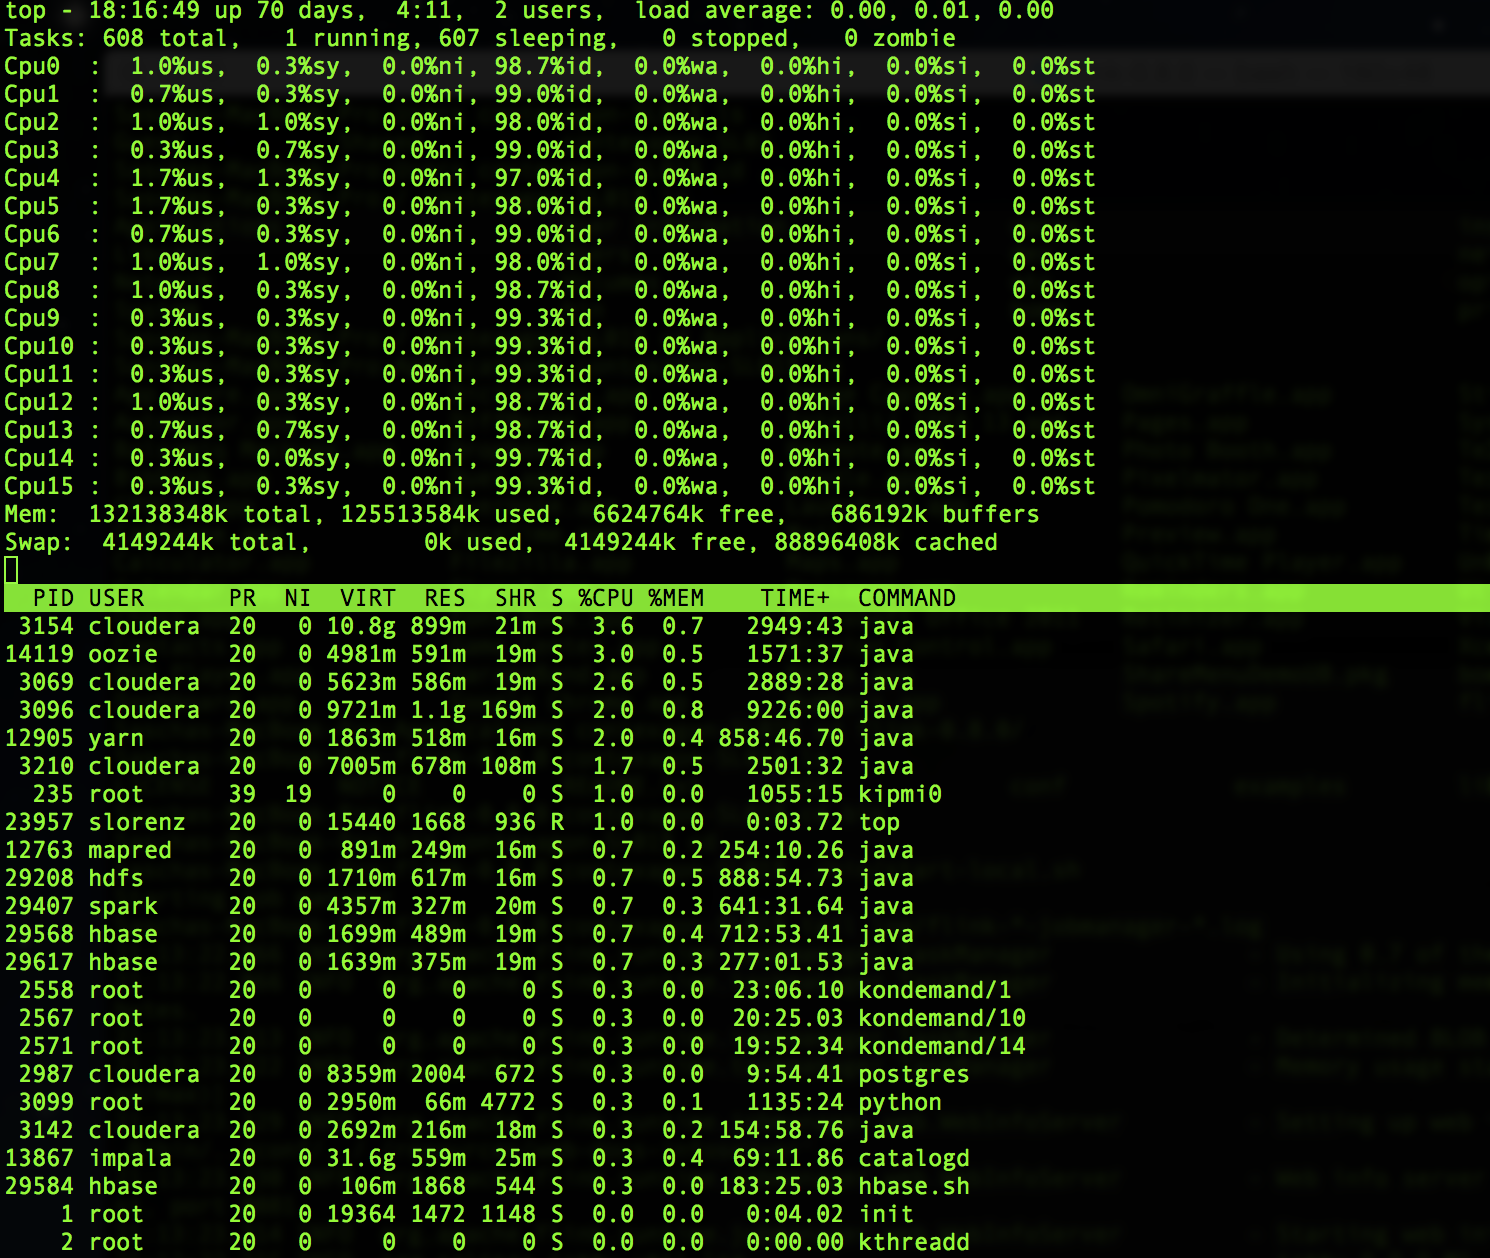
\includegraphics[width=1.0\textwidth]{bilder/top_cluster.png}
\caption{Ausführung des Linux-Befehls top auf dem Master-Node des Beuth-Clusters.}
\label{fig:topcluster}
\end{figure}    

Eine Einschränkung dieses Kommandos ist die fehlende Identifikation der benutzten Prozessorkerne bei Verwendung von Multicore-Systemen. Die prozentuale Prozessorauslastung wird pro Kern angegeben. Am Beispiel des unter anderem eingesetzten MacBook Pro mit i7 Prozessor (vier physische Kerne, acht mit Hyperthreading) bedeutet dies, dass eine Maximalauslastung der CPU bei dieser Metrik einen Wert von 800\% erreicht. Außerdem lässt sich bei einer dargestellten Auslastung von 100\% so nicht ermitteln, ob es sich bei diesem Wert um einen Thread mit 100\% Auslastung eines Kernes, um zwei Threads mit 80\% und 20\%, oder um vier unabhängige Threads mit je 25\% Kernauslastung handelt. Aus diesem Grund werden für die Metriken statt der prozentualen Angabe der CPU-Auslastung die CPU-Zeit als Messgrößen verwendet. Diese ist proportional zur Prozessorauslastung. Für die durchgeführten Vergleichsmessungen werden die CPU-Zeiten der Standardimplementierung des BDAS mit 100\% gewertet und die Vergleichsalgorithmen dazu in ein Verhältnis gesetzt.  

Da Spark die RDDs wenn möglich im Hauptspeicher hält und nur auf Festspeicher auslagert, wenn das RAM nicht ausreichend ist, wird auf ein Monitoring des Hauptspeichers für diese Messungen verzichtet. Statt dessen werden die I/O-Vorgänge überwacht um so einen Überlauf auf den Festspeicher und damit begründete Performance-Einbrüche feststellen zu können. 

\section{Beschreibung der Messumgebungen}
\label{section:messumgebungen}

Zum Einsatz für die Evaluierung kamen für diese Untersuchung unterschiedliche Ansätze für Clusterinfrastrukturen. Es kamen diverse lokale Installationen, sowie ein leistungsfähiges Rechnercluster an der Beuth Hochschule Berlin zum Einsatz.  

Die Tabelle \ref{tab:lokale hardware} gibt eine detaillierte Übersicht über die lokal verwendeten Hardwarekonfigurationen. Alle lokal eingesetzten Maschinen verfügen über SSDs (Solid State Drives) als Festspeicher.

\begin{table}[!ht]
\centering
\begin{tabular}{| p{3cm} | p{2.2cm} |  p{3cm} |  p{1.2cm} | p{3cm} | }
\hline
System & CPU & Anzahl Cores & RAM & OS\\ \hline \hline
MacBook Pro Mid 2014 & Intel i7 & 4 physisch, 8 mit Hyperthreading & 16 GB & Mac OS-X 10.10.2 Yosemite \\ \hline
Apple iMac Mid 2011 & Intel i5 & 4 physisch, 8 mit Hyperthreading & 16 GB & Mac OS-X 10.10.2 Yosemite \\ \hline
Xeon Workstation & Intel Xeon 1230 & 4 physisch, 8 mit Hyperthreading & 32 GB & Windows 8.1,  VirtualBox Instanzen mit CentOS  \\ \hline 
Lenovo ThinkPad 410T & Intel i5 & 4 physisch & 8 GB & Windows 8.1, VirtualBox Instanzen mit CentOS  \\ \hline 

\end{tabular}
\caption{Übersicht der lokal verwendeten Hardware}
	\label{tab:lokale hardware}
\end{table}  

Die Tabelle \ref{tab:cluster} zeigt die Konfiguration (Konfigurationsstand Dezember 2014) des verwendeten Clustersystems an der Beuth Hochschule Berlin. 

\begin{table}[!ht]
\centering
\begin{tabular}{| p{3cm} | p{2.2cm} |  p{3cm} |  p{1.2cm} | p{3cm} | }
\hline
System & CPU & Anzahl Cores & RAM & OS\\ \hline \hline
Master Node & AMD 6320 & 2 * 8  & 128 GB & Debian Linux \\ \hline
Worker Node 1 & AMD 6378 & 4 * 16 & 512 GB &  Debian Linux\\ \hline
Worker Node 2 & AMD 6378 & 4 * 16 & 512 GB &  Debian Linux\\ \hline
Worker Node 3 & AMD 6378 & 4 * 16 & 512 GB &  Debian Linux\\ \hline

\end{tabular}
\caption{Übersicht über das Cluster der Beuth Hochschule Berlin}
	\label{tab:cluster}
\end{table}  

\subsection{Lokales Single Node Cluster  }
\label{section:lokales single node}

TBD!

\subsection{Lokales Multi Node Cluster}
\label{section:tachyon}

TBD!

\subsection{Remote Cluster an der Beuth Hochschule}
\label{section:remote}

TBD!

\section{Ergebnisse}
\label{section:ergebnisse}

TBD!

\subsection{Messergebnisse Apache Spark}
\label{section:spark eval}

TBD!

\subsection{Messergebnisse Apache Flink}
\label{section:mllib arch}

TBD!

\subsection{Messergebnisse MLLib}
\label{section:mllib arch}

TBD!

\subsection{Messergebnisse H2O}
\label{section:mllib arch}

TBD!



\section{Zusammenfassung}
\label{section:zusammen}



TBD!
